% DPF 09 talk on strangeness in nucleon

\documentclass[10pt]{beamer}
\usepackage{amsmath}
\usepackage{mathtools}
\usefonttheme{professionalfonts} % using non standard fonts for beamer
\usefonttheme{serif} % default family is serif
%\documentclass[12pt]{beamerthemeSam.sty}
\usepackage{epsf}
%\usepackage{pstricks}
%\usepackage[orientation=portrait,size=A4]{beamerposter}
\geometry{paperwidth=160mm,paperheight=120mm}
%DT favorite definitions
\def\LL{\left\langle}	% left angle bracket
\def\RR{\right\rangle}	% right angle bracket
\def\LP{\left(}		% left parenthesis
\def\RP{\right)}	% right parenthesis
\def\LB{\left\{}	% left curly bracket
\def\RB{\right\}}	% right curly bracket
\def\PAR#1#2{ {{\partial #1}\over{\partial #2}} }
\def\PARTWO#1#2{ {{\partial^2 #1}\over{\partial #2}^2} }
\def\PARTWOMIX#1#2#3{ {{\partial^2 #1}\over{\partial #2 \partial #3}} }

\def\rightpartial{{\overrightarrow\partial}}
\def\leftpartial{{\overleftarrow\partial}}
\def\diffpartial{\buildrel\leftrightarrow\over\partial}

\def\BC{\begin{center}}
	\def\BS{\bigskip}
\def\EC{\end{center}}
\def\BI{\begin{itemize}}
\def\EI{\end{itemize}}
\def\BE{\begin{displaymath}}
\def\EE{\end{displaymath}}
\def\BEA{\begin{eqnarray*}}
\def\EEA{\end{eqnarray*}}
\def\BNEA{\begin{eqnarray}}
\def\ENEA{\end{eqnarray}}
\def\EL{\nonumber\\}


\newcommand{\etal}{{\it et al.}}
\newcommand{\gbeta}{6/g^2}
\newcommand{\la}[1]{\label{#1}}
\newcommand{\ie}{{\em i.e.\ }}
\newcommand{\eg}{{\em e.\,g.\ }}
\newcommand{\cf}{cf.\ }
\newcommand{\etc}{etc.\ }
\newcommand{\atantwo}{{\rm atan2}}
\newcommand{\Tr}{{\rm Tr}}
\newcommand{\dt}{\Delta t}
\newcommand{\op}{{\cal O}}
\newcommand{\msbar}{{\overline{\rm MS}}}
\def\chpt{\raise0.4ex\hbox{$\chi$}PT}
\def\schpt{S\raise0.4ex\hbox{$\chi$}PT}
\def\MeV{{\rm Me\!V}}
\def\GeV{{\rm Ge\!V}}


%AB: my color definitions
\definecolor{A}{rgb}{0.8,0.0,0.0}
\definecolor{B}{rgb}{0.0,0.6,0.0}
\definecolor{C}{rgb}{0.6,0.6,0.0}
\definecolor{D}{rgb}{0.0,0.0,0.5}
\definecolor{E}{rgb}{0.4,0.4,0.4}

%\definecolor{mygarnet}{rgb}{0.445,0.184,0.215}
%\definecolor{mygold}{rgb}{0.848,0.848,0.098}
%\definecolor{myg2g}{rgb}{0.647,0.316,0.157}
\definecolor{abtitlecolor}{rgb}{0.0,0.255,0.494}
\definecolor{absecondarycolor}{rgb}{0.0,0.416,0.804}
\definecolor{abprimarycolor}{rgb}{1.0,0.686,0.0}
\definecolor{Red}           {cmyk}{0,1,1,0}
\definecolor{Grey}           {cmyk}{.7,.7,.7,0}
\definecolor{Blue}          {cmyk}{1,1,0,0}
\definecolor{Green}         {cmyk}{1,0,1,0}
\definecolor{Brown}         {cmyk}{0,0.81,1,0.60}

\usetheme{Madrid}


%AB: redefinition of beamer colors
%\setbeamercolor{palette tertiary}{fg=white,bg=mygarnet}
%\setbeamercolor{palette secondary}{fg=white,bg=myg2g}
%\setbeamercolor{palette primary}{fg=black,bg=mygold}
\setbeamercolor{title}{fg=abtitlecolor}
\setbeamercolor{frametitle}{fg=abtitlecolor}
\setbeamercolor{palette tertiary}{fg=white,bg=abtitlecolor}
\setbeamercolor{palette secondary}{fg=white,bg=absecondarycolor}
\setbeamercolor{palette primary}{fg=black,bg=abprimarycolor}
\setbeamercolor{structure}{fg=abtitlecolor}

\setbeamerfont{section in toc}{series=\bfseries}

%AB: remove navigation icons
\beamertemplatenavigationsymbolsempty
\title[1D kinematics]{
  \textbf {1D kinematics: solving problems} 
%\centerline{}
%\centering
%\vspace{-0.0in}
%\includegraphics[width=0.3\textwidth]{propvalues_0093.pdf}
%\vspace{-0.3in}\\
%\label{intrograph}
}

\author[W. Freeman] {Physics 211\\Syracuse University, Physics 211 Spring 2021\\Walter Freeman}

\date{\today}

\begin{document}

\frame{\titlepage}

\frame{\frametitle{\textbf{On solving problems}}
\large
\begin{center}
\color{Red}
You can recognize truth by its beauty and simplicity. 
When you get it right, it is obvious that it is right--at least if you have any experience--because 
usually what happens is that more comes out than goes in....
Inexperienced students make guesses that are very complicated, $[$but$]$ the truth always turns out to be simpler than you thought.

\bigskip

\end{center}
\bigskip
--Richard Feynman, quoted by K. C. Cole, in {\it Sympathetic Vibrations: Reflections on Physics as a Way of Life (1985)}

\bigskip
\bigskip
\bigskip
\bigskip

\begin{center}
\color{Red}
Nature uses only the longest threads to weave her patterns, so each small piece of her fabric reveals the organization of the entire tapestry.
\bigskip

\end{center}
\bigskip
--Richard Feynman, {\it The Character of Physical Law} (1965) 



}



\frame{\frametitle{\textbf{Announcements}}
\large
\BI
\item{Homework 1 due tomorrow}\pause
\item Lots of opportunities for you to seek and receive help \pause
\BI
\item What happened in the Virtual Clinic yesterday? \pause
\item My Clinic hours today: 3:30-5:30
\item Many other people have other hours -- see the course website
\EI
\item Lively discussion going on on the course Discord server about the homework

\BS
\BS

\item Homework 2 will be posted tomorrow and due next Thursday before class
\EI
}



\frame{\frametitle{\textbf{Quiz 1}}
Quiz 1 will be next Thursday. {\color{Green}Don't panic!} -- you'll be fine!

\BS\BS

\pause
There will be {\it two questions}. On the quiz:
\BI
\item One question where you will need to interpret the two roots given to you by the quadratic formula (like Question 5 from HW1)
\BS
\item Motion with constant acceleration in one dimension (what you did for HW1: roadrunner problem, elevator problem)
\BS
\item Motion with constant acceleration in two dimensions (what we are doing today and next Tuesday, and on HW2: cannon problem, dog problem)
\BS
\item Interpretation of position/velocity/acceleration graphs (HW1, bicycle problem)
\EI
\pause
}

\frame{\frametitle{\textbf{Quiz 1}}
\BS
Review opportunities specifically for the quiz:

\BI
\item next Wednesday, 4PM-7PM, on Zoom (link provided next week)
\item next Thursday, first 20 minutes of class
\EI

\BS
The quiz itself:
\BI
\item A PDF will be posted at 11:20 AM on the website and on Blackboard; it will be due at 12:20 PM (end of class). We will have a grace period to accommodate people scanning and submitting things.

\BS

\item Four options to take it:
\begin{enumerate}
	\item Write the answers on your own paper, scan them, and submit them
	\item Print the PDF, write the answers on it, scan it, and submit it
	\item Write the answers on the PDF using a tablet and submit a PDF
	\pause
	\item Limited capacity to take the quiz in person; if you might be interested, tell me now (gauging interest; instructions to come)
	\pause
	ODS students will get extra time; we'll figure that out and give you instructions next week.
	\end{enumerate}
\EI
}


\frame{\frametitle{\textbf{Vectors}}
	\large
	You've been doing math with numbers, which are things that live in one dimension: they only have a magnitude and a sign.
	
	\bigskip
	\bigskip
	
	Vectors are things that have a magnitude and a direction: ``arrows in space''
	
	\bigskip
	\bigskip
	
	Many of the things we deal with in physics are vectors:
	\BI
	\item{{\color{Red}Position}}
	\pause
	\item{(and its derivatives: {\color{Red}velocity} and {\color{Red}acceleration})}
	\pause
	\item{{\color{Red}Force, momentum}}
	\EI
	\bigskip
	\bigskip
	\pause
	So, we need to learn to do math with arrows.
	\BI
	
	\item{We indicate that an object is a vector by writing an arrow over it: ``the vector $\vec V$''.}
	\item{``Scalar'': object that isn't a vector (mass, time)}
	\item{Equations can mix vectors and scalars: $\vec F = m \vec a$.}
	\item{... or $\vec s = \frac{1}{2}\vec a t^2 + \vec v_0 t + \vec s_0$}
	\EI
}

\frame{\frametitle{\textbf{Notation}}
	
	\Large
	
	\BI
	\item $\vec A$: ``the vector A'' (a vector)
	\item $A$: ``the magnitude of A'' (a scalar)
	\item $\hat A$: ``the direction A points in'' (a vector with magnitude 1)
	\item $A_x$: the component of A along the $x-$axis (a scalar)
	\item $A_y$: the component of A along the $y-$ayis (a scalar)
	\EI
}

\frame{\frametitle{\textbf{Two ways to describe a vector}}
	\begin{columns}
		\column{0.5\textwidth}
		\centerline{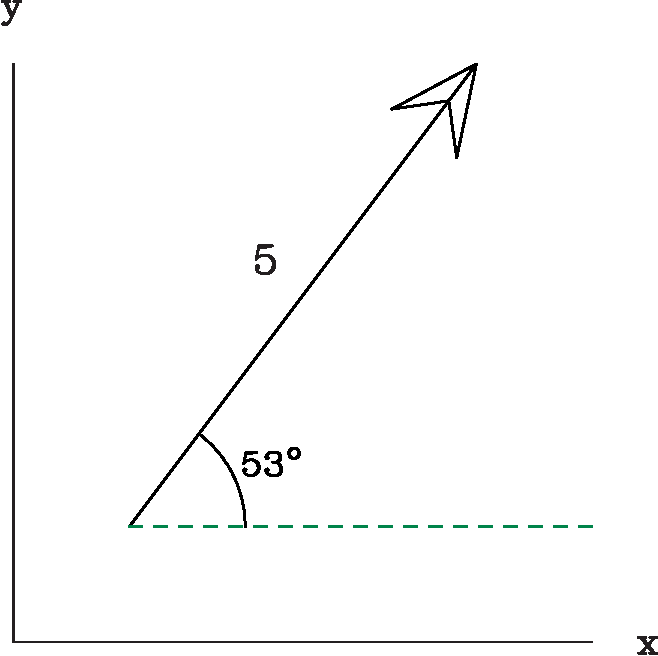
\includegraphics[width=0.7\textwidth]{vector-angle-crop.pdf}}
		\Large
		\centerline{Angle and direction}
		\column{0.5\textwidth}
		\centerline{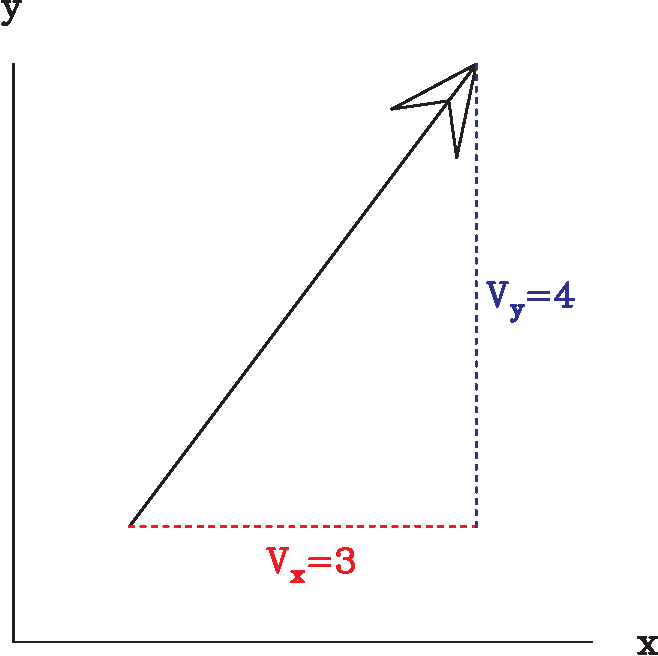
\includegraphics[width=0.7\textwidth]{vector-components-crop.pdf}}
		\Large
		\centerline{X and Y components}
	\end{columns}
	\bigskip
	\bigskip
	\Large
	\centerline{How do we convert from one to the other?}
}


\frame{\frametitle{\textbf{How do we convert from one to the other?}}
	
	\Huge
	
	A: Using algebra\\
	B: Using trigonometry\\
	C: Using calculus\\
	D: Using differential equations\\
}

\frame{\frametitle{\textbf{From ``direction and magnitude'' to components}}
	\centerline{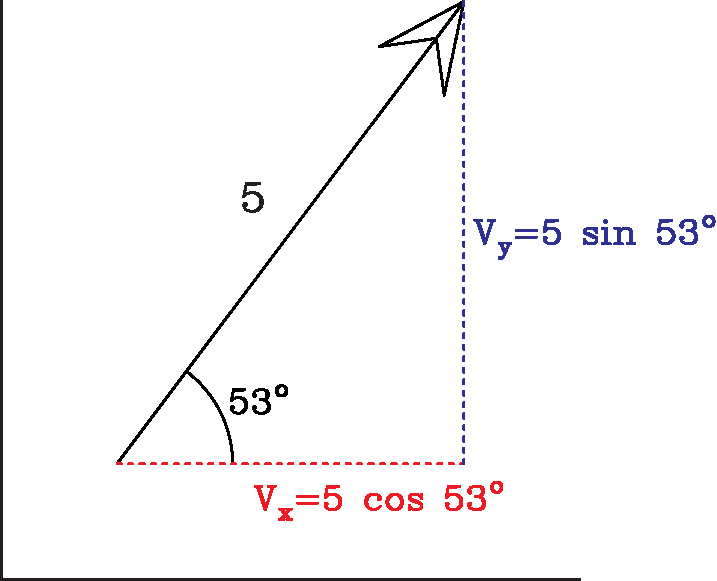
\includegraphics[width=0.6\textwidth]{vector-ang2comp-crop.pdf}}
}

\frame{\frametitle{\textbf{From components to direction and magnitude}}
	\centerline{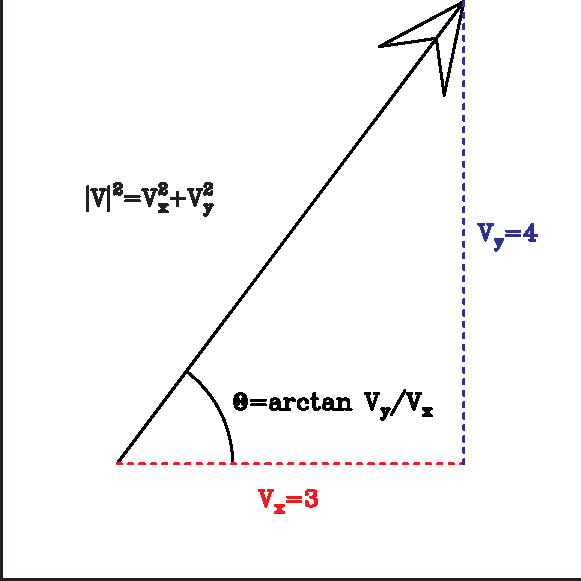
\includegraphics[width=0.6\textwidth]{vector-comp2ang-crop.pdf}}
}

\frame{
	
	\Huge
	
	Suppose you have some vector $\vec A$ that you want to convert into components.
	The $x$-component $A_x$ is:
	
	\bigskip
	
	A: $A \cos \theta$\\
	B: $A \sin \theta$\\
	C: $A \tan \theta$\\
	D: $\frac{A}{\cos \theta}$\\
	E: It depends
	
}

\frame{\frametitle{\textbf{A warning!}}
	
	\centerline{\Large{You cannot memorize ``$V \sin \theta$ is the $y$ component,}}  
	\centerline{\Large{$V \cos \theta$ is the $x$ component''!}}
	\bigskip
	\bigskip
	\centerline{\Large{This does {\it not} work in general; you have to actually draw the triangle.}}
}

\frame{\frametitle{\textbf{Adding vectors}}
	We can also add vectors together by drawing them ``head to tail''. Here are two vectors:
	
	\bigskip
	\bigskip
	
	\begin{columns}
		\column{0.5\textwidth}
		\centerline{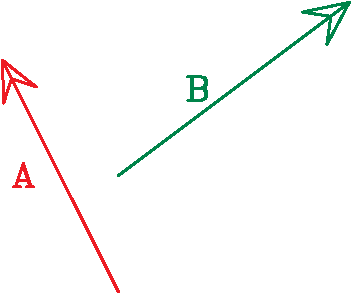
\includegraphics[width=0.6\textwidth]{vshow-crop.pdf}}
		\column{0.5\textwidth}
		\centerline{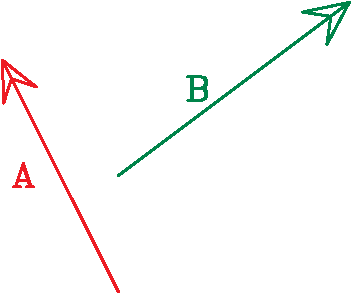
\includegraphics[width=0.6\textwidth]{vshow-crop.pdf}}
	\end{columns}
}

\frame{
	\centerline{\Large Does $\vec A + \vec B = \vec B + \vec A$?}
	
	\bigskip
	\bigskip
	\bigskip
	
	\Large
	
	\BI
	\item{A: Yes}
	\item{B: No}
	\EI
	
	\pause
	
	\bigskip
	\bigskip
	\bigskip
	
	Yes: vector addition obeys the commutative property, just like ordinary addition
}

\frame{\frametitle{\textbf{Adding vectors}}
	\centerline{We can also add vectors together by drawing them ``head to tail''. Here are two vectors:}
	
	\bigskip
	\bigskip
	
	\begin{columns}
		\column{0.5\textwidth}
		\centerline{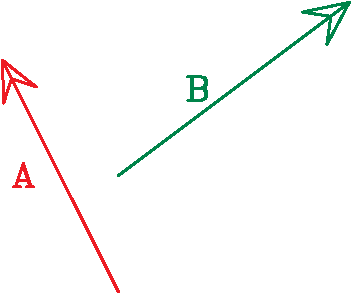
\includegraphics[width=0.6\textwidth]{vshow-crop.pdf}}
		\column{0.5\textwidth}
		\centerline{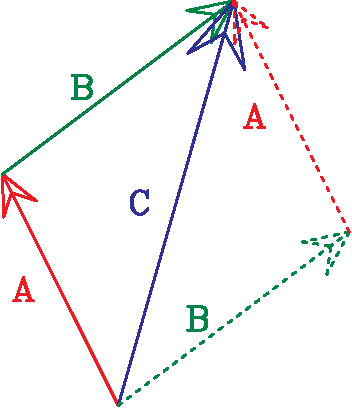
\includegraphics[width=0.6\textwidth]{vadd-crop.pdf}}
	\end{columns}
	
	\bigskip
	\bigskip
	
	\Large \centerline{$\color{Red}\vec A + \color{Green} \vec B = \color{Blue} \vec C$}
	
}

\frame{\frametitle{\textbf{Adding vectors: components}}
	\centerline{\Large The component representation is much easier to work with!}
	
	\Huge\centerline{$\color{Red}\vec A + \color{Green} \vec B = \color{Blue} \vec C \color{Black} \rightarrow {\color{Red} A_x + \color{Green} B_x = \color{Blue} C_x \choose \color{Red} A_y + \color{Green} B_y = \color{Blue} C_y}$}
}

\frame{\frametitle{\textbf{Adding vectors: components}}
	\centerline{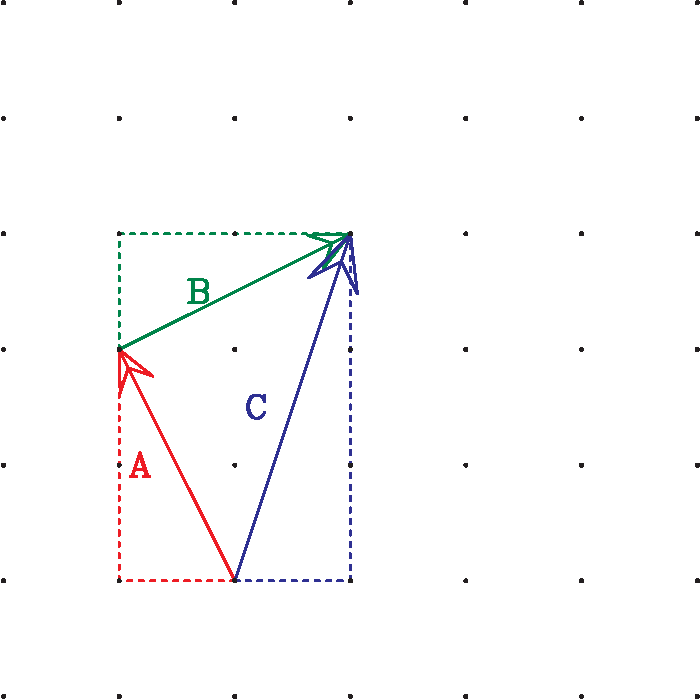
\includegraphics[width=0.4\textwidth]{vaddc-crop.pdf}}
	
	\large
	\bigskip
	
	\centerline{To add two vectors, just add their components!}
	
	\bigskip
	
	\centerline{This is why it is almost always easiest to work in the component representation!}
}

\frame{\frametitle{\textbf{What does this do to our kinematics?}}
	\large Acceleration, velocity, and position relationships are still the same; they just apply {\color{Red}independently} for each component.
	\Large
	
	\begin{align*}
	\vec v(t) =&\, \vec at + \vec v_0 \\
	\vec s(t) =&\, \frac{1}{2}\vec a t^2 + \vec v_0 t + \vec s_0
	\end{align*}
	
	\pause
	
	\begin{align*}
	\vec v_x(t) =&\, a_x t + v_{x,0} \\
	\vec v_y(t) =& a_y t + v_{y,0} \\
	\end{align*}
	\pause
	\begin{align*}
	\vec x(t) =&\,  \frac{1}{2}  a_x t^2 + v_{x,0} t + x_0\\
	\bigskip
	\vec y(t) =&\, \frac{1}{2}  a_y t^2 + v_{y,0} t + y_0
	\end{align*}
}


\frame{
	\centerline{\Large Which statement does {\it not} make sense?} 
	
	\bigskip
	\bigskip
	\bigskip
	
	\Large
	
	\BI
	\item{a. $\vec A t = \vec B$}
	\item{b. $\vec A + \vec B + t = \vec C$}
	\item{c. $k(\vec A + \vec B) = k\vec A + k\vec B$}
	\item{d. $\vec A - \vec B = \vec C$}
	\EI
	
	\pause
	
	\bigskip
	\bigskip
	\bigskip
	
	B: You can't add a vector and a scalar. ``One mile north plus one inch'' -- which way is the inch?
}

\frame{\frametitle{\textbf{Problem solving: 2D kinematics, constant acceleration}}
	\Large
	\begin{enumerate}
		\item{1. If you have vectors in the ``angle and magnitude'' form, convert them to components}
		\item{2. Write down the kinematics relations, separately for $x$ and $y$}
		\begin{itemize}
			\large
			\item{Many terms will usually be zero}
			\item{Freefall: $a_x = 0$, $a_y = -g$ (with conventional choice of axes)}
		\end{itemize}
		\item{3. Understand what instant in time you want to know about}
		\item{4. Put in what you know; solve for what you don't (using substitution, if necessary)}
		\item{5. Convert vectors into whatever format the problem asks for}
	\end{enumerate}
	\pause
	
	\bigskip
	\bigskip
	
	
	
	\centerline{\Large{\color{Red}Every kinematics problem we will encounter can be done this way!}}
}

\frame{\frametitle{\textbf{Sample problems}}
	\centerline{\Large{A rock is thrown at $v_0=10 m/s$ at $\theta=30^\circ$ above the horizontal.}}
	
	\bigskip
	\bigskip
	
	\begin{itemize}
		\large
		\item{How far from its starting point is it after 2 seconds?}
		\pause
		\item{How far does it travel?}
		\pause
		\item{How high does it go?}
		\pause
		\item{What will its speed be when it strikes the ground?}
	\end{itemize}
}




\end{document}

